\subchapter{Init script optimizations}{Analyzing and optimizing init
scripts}

\section{Measuring}

Remember that the first step in optimization work is measuring elapsed
time. We need to know which parts of the init scripts are the biggest
time consumers.

Check and write down the initial size of the root filesystem archive.

\subsection{Use bootchartd on the board}

Add \code{bootchartd} support (\projconfig{busybox}{CONFIG_BOOTCHARTD})
to your \code{BusyBox} configuration:

\begin{verbatim}
cd ~/boot-time-labs/rootfs/buildroot
make busybox-menuconfig
\end{verbatim}

In \code{Archival Utilities}, also enable \code{Make tar, rpm, modprobe
etc understand .gz data} (\code{FEATURE_SEAMLESS_GZ}), which is needed by
\code{bootchartd}.

After saving the configuration, the \code{make} command should only take
a few seconds to run.

\subsection{Re-flash the root filesystem}

Update your root filesystem on the SD card.

The next thing to do is to use the \code{init} argument on the
kernel command line (in \code{u-boot}, this is the \code{bootargs}
environment variable) to boot using \code{bootchart} instead of using
the \code{init} program provided by Busybox.

So, boot your board but stay in the U-Boot shell, by pressing the
\code{Space} key before the timer expires.

Add \code{init=/sbin/bootchartd} to the bootargs variable:
\begin{verbatim}
U-Boot> setenv bootargs ${bootargs} init=/sbin/bootchartd
U-Boot> saveenv
\end{verbatim}

This will make the system boot and the resulting bootlog will be located
in \code{/var/log/bootlog.tgz}. As \code{/var/log} is actually stored in
RAM (through the {\em tmpfs} filesystem, you will copy it to the root
filesystem.

First, as the filesystem is read-only, remount it in read-write mode:
\begin{verbatim}
mount -o remount,rw /
\end{verbatim}

Now, copy the file to the root filesystem storage and halt your board:

\begin{verbatim}
cp /var/log/bootlog.tgz /root/
halt
\end{verbatim}

Remove the SD card, insert it in your PC, and copy that file on your host:

\begin{verbatim}
cd $HOME/boot-time-labs/rootfs
sudo cp /media/$USER/rootfs/root/bootlog.tgz .
sudo chown $USER.$USER bootlog.tgz
\end{verbatim}

\subsection{Analyze bootchart data on your workstation}

To compile and use \code{bootchart} on your workstation, you first need to
install a few Java packages:

\begin{verbatim}
sudo apt install ant openjdk-11-jdk
\end{verbatim}

Note that \code{ant} is a Java based build tool like \code{make}.

Now, get the \code{bootchart} source code for version 0.9 from
\url{https://bootlin.com/pub/source/bootchart-0.9.tar.bz2}\footnote{Don't try to get the \code{bootchart} package supplied by
Ubuntu instead. While it has similar functionality, it looks like a completely
unrelated piece of software. To confirm this, it has no dependency
whatsoever on Java packages.}, compile it and use \code{bootchart} to generate the boot
chart:

\begin{verbatim}
tar xf bootchart-0.9.tar.bz2
cd bootchart-0.9
ant
java -jar bootchart.jar ~/boot-time-labs/rootfs/bootlog.tgz
\end{verbatim}

This produces the \code{bootlog.png} image which you can visualize to
study and optimize your startup sequence:

\begin{verbatim}
xdg-open bootlog.png
\end{verbatim}

\code{xdg-open} is a universal way of opening a file with a given MIME
type with the associated application as registered in the system.
According to the exact Ubuntu flavor that you are using,
it will run the particular image viewer available in that
particular flavor.

\begin{center}
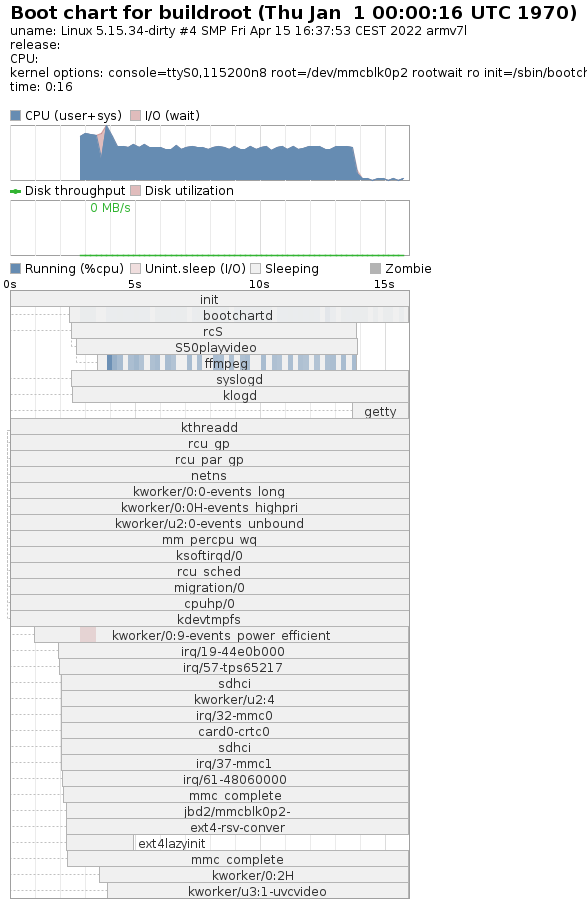
\includegraphics[height=8cm]{labs/boot-time-init-scripts/bootlog.png}
\end{center}

\section{Remove unnecessary functionality}

\subsection{Getting Buildroot to generate less files}

The above graph shows several system processes running
during the startup process, consuming CPU time, probably delaying
the execution of our application (see the color bars showing when
a task is using the CPU).

In the general case, there will be services that you want to keep. At
least, you could change the order according to which services are
started, by changing the alphanumeric order of startup files (that's
reordering / postponing work).

Back to our case, we want to simplify our system as much as possible.
In Buildroot's configuration interface, go to the \code{System
Configuration} menu:

\begin{itemize}
\item Disable \code{Enable root login with password} and
      \code{Run a getty (login prompt) after boot}.
\item Disable \code{Purge unwanted locales}
\end{itemize}

Don't forget to remove \code{bootchartd} support as well and
\code{BR2_FEATURE_SEAMLESS_GZ} which we added earlier.
Also disable \code{ifupdown scripts} in \code{Networking applications}.
This allows to remove the \code{/etc/init.d/S40network} script.

Before we update the filesystem, let's make another experiment: boot
your board, interrupt the video player, and unmount \code{/proc} and
\code{/sys} manually. Then, run the video player command again, and
you'll see that \code{ffmpeg} runs perfectly without these virtual
filesystems mounted.

This means we could directly run the video player as the {\em init}
process! To keep the possibility to interact with the board through
a command line shell, we're going to run a shell after the video player.

So, let's remove \code{/etc/init.d/S50playvideo} from the root
filesystem overlay and replace it by the \code{/playvideo} script
provided in \code{~/boot-time-labs/rootfs/data/}.

Regenerate your root filesystem:
\begin{verbatim}
make clean
make
\end{verbatim}

Update and reflash your SD card. Reboot the board, but before booting,
stop in U-Boot to update the {\em init} program:

\begin{verbatim}
setenv bootargs console=ttyS0,115200n8 root=/dev/mmcblk0p2 rootwait rw init=/playvideo
saveenv
boot
\end{verbatim}

Note that the \code{rw} setting is going to be important, as it will
make Linux mount the root filesystem in read/write mode, which allows to
record the access time of each file.

\subsection{Detecting and eliminating unused files}

If the video played ran fine as expected, you should now be in a shell
in the serial console.

Type the \code{sync} command to flush the filesystem, remove the SD card
and insert it on your PC again. Go to \code{/media/$USER/rootfs} and run
the below command:

\begin{verbatim}
find . -atime -100 -type f
\end{verbatim}

This lists the regular files that were not accessed during the boot
sequence we've just executed:

\begin{verbatim}
./usr/lib/os-release
./usr/share/ffmpeg/libvpx-720p50_60.ffpreset
./usr/share/ffmpeg/libvpx-360p.ffpreset
./usr/share/ffmpeg/libvpx-720p.ffpreset
./usr/share/ffmpeg/ffprobe.xsd
./usr/share/ffmpeg/libvpx-1080p.ffpreset
./usr/share/ffmpeg/libvpx-1080p50_60.ffpreset
./usr/share/udhcpc/default.script
./bin/busybox
./lib/libatomic.so.1.2.0
./lib/libgcc_s.so.1
./etc/hostname
./etc/profile.d/umask.sh
./etc/init.d/S02klogd
./etc/init.d/S20urandom
./etc/init.d/rcS
./etc/init.d/rcK
./etc/init.d/S01syslogd
./etc/group
./etc/protocols
./etc/inittab
./etc/passwd
./etc/services
./etc/fstab
./etc/shadow
./etc/hosts
./etc/profile
./etc/issue
./etc/shells
\end{verbatim}

How does it work?

\code{-atime -100} finds all the files which last access time is
less than 100 minutes ago, actually when we extracted the archive.
Why doesn't it find the files which were actually accessed during the
boot sequence? That's because the board doesn't have a clock set and its
date got back to January 1st, 1970. You can check the date of such a
file:

\begin{verbatim}
stat etc/init.d/playvideo
  File: etc/init.d/playvideo
  Size: 300       	Blocks: 8          IO Block: 4096   regular file
Device: b302h/45826d	Inode: 376         Links: 1
Access: (0755/-rwxr-xr-x)  Uid: ( 1000/    mike)   Gid: ( 1000/    mike)
Access: 1970-01-01 01:00:02.250000000 +0100
Modify: 2019-05-21 22:29:21.348835786 +0200
Change: 2019-05-21 22:29:21.748834877 +0200
 Birth: -
\end{verbatim}

A limitation is that it doesn't work with symbolic links and directories, so we don't
know whether a symbolic link or directory was accessed or not. That's why we're
keeping only regular files (\code{-type f}).

There's a discrepancy too with \code{/bin/busybox} which was for sure
accessed, but through a symbolic link. We will have to remove it from
the list.

If we had a board with a correct date, we would have still been able to
use this technique, but this time only looking for files last accessed more
than a few minutes ago (\code{-atime +5}).

We can now implement a Buildroot {\em Post build script} that will
eliminate such files in the target directory. That's much easier than
tweaking the recipes that generated these files, and this can be adapted
to each case (each case is special, while recipes should be generic).

So, in the Buildroot directory, create a
\code{board/beaglecam/post-fakeroot.sh} script that removing all the above
files (except \code{/bin/busybox}):

\begin{verbatim}
#!/bin/sh
TARGET_DIR=$1
cd $TARGET_DIR
rm -rf \
./usr/lib/os-release \
./usr/share/ffmpeg/libvpx-720p50_60.ffpreset \
./usr/share/ffmpeg/libvpx-360p.ffpreset \
...
\end{verbatim}

Don't forget to make this script executable!

The last thing to do is to configure \code{BR2_ROOTFS_POST_FAKEROOT_SCRIPT}
to \code{board/beaglecam/post-fakeroot.sh}\footnote{We could have used
Buildroot's post build scripts (\code{BR2_ROOTFS_POST_BUILD_SCRIPT}),
but that would have been too early, as the \code{fakeroot} scripts make
some customizations on files like \code{/etc/inittab}, which we want
to remove.}.

Rerun Buildroot and check that your root filesystem was simplified as
expected:

\begin{verbatim}
make
\end{verbatim}

See what's left in the final archive. Actually, we propose to be more
aggressive and directly remove the entire \code{/etc} directory which we
shouldn't need any more. Do the same for \code{/root}, \code{/tmp},
\code{/var}, \code{/media}, \code{/mnt}, \code{/opt}, \code{/run} and
the \code{/lib32} link. We're keeping the \code{/proc} and \code{/sys}
directories in case we need to mount the corresponding filesystems.

Why doing this so aggressively for files we won't access? On an {\em
ext4} filesystem, files that are not accessed may not do any harm if
they are not used, except perhaps marginally in terms of mounting time
(if the filesystem is unnecessarily big). However, if we store the root
filesystem in an {\em Initramfs} embedded in the kernel binary,
every byte counts as it will make the kernel to load bigger.

Update your root filesystem, remove the \code{rw} kernel parameter from
\code{bootargs} in U-Boot (better to keep the root filesystem mounted read-only as we don't
cleanly shut down the system) and check that your system still boots fine.

Check and write down the new size of the root filesystem archive.

\subsection{Reducing BusyBox to the minimum}

While we're simplifying the root filesystem, it's time to reduce the
configuration of Busybox, to only contain the features we need in our
system.

Before we do this, check the size of the \code{busybox} executable in
your root filesystem.

Buildroot helps us to configure BusyBox by providing a \code{make
busybox-menuconfig} command, but it will be tedious to use because we
will have to unselect countless options.

Here's another way. Go to \code{output/build/busybox-1.29.3/} and run
\code{make allnoconfig}, followed by \code{make menuconfig}. You'll see
that most options are unselected!

Just select the below options, based on what we have in our
\code{/playvideo} script:
\begin{itemize}
  \item In \code{Settings}:
  \begin{itemize}
     \item Enable \code{Support files > 2 GB}. Without this, BusyBox
           will fail to compile (at least with our toolchain)
  \end{itemize}
  \item In \code{Shells}:
  \begin{itemize}
     \item Enable \code{Use internal glob() implementation}, even
	   if you don't select \code{ash}. Otherwise, compiling
           \code{hush} will fail.
     \item Select the \code{hush} shell
     \item Keep only \code{Support if/then/elif/else/fi} and
           \code{Support for, while and until loops},
  \end{itemize}
  \item In \code{Coreutils}:
  \begin{itemize}
     \item Support for the \code{sleep} command, with support for fractional arguments.
     \item Support for the \code{echo} command, without additional options.
     \item Enable \code{test} and \code{test as [}
     \item Disable \code{Extend test to 64 bit}
  \end{itemize}
\end{itemize}

Now get back to the main Buildroot directory and copy this new
configuration:

\begin{verbatim}
cp output/build/busybox-1.31.1/.config board/beaglecam/busybox.config
\end{verbatim}

Then, run \code{make menuconfig} and set
\code{BR2_PACKAGE_BUSYBOX_CONFIG} to this new file. In \code{System
configuration}, also set \code{Init system} to \code{None}. Otherwise
Buildroot will enable Busybox \code{init} into your configuration.

Run \code{make}, and update your SD card.
Check the new size of \code{/bin/busybox}!

Also write down the new size of the root filesystem tar archive.

\subsection{Switching to static executables}

Since we now have only two executables (\code{busybox} and
\code{ffmpeg}), let's explore the possibility to switch to static
executables, hoping to reduce filesystem size by not having to copy
the entire shared libraries.

In Buildroot's configuration interface, find and set
\code{BR2_STATIC_LIBS=y}.

Run \code{make clean} and \code{make}.

Run \code{tar tvf output/images/rootfs.tar} to find out directories
which are now empty and therefore can now be removed. Add such directories to
your post-fakeroot script and regenerate the filesystem again.
This should save a few extra bytes.

Once more, write down the new size of the root filesystem tar archive.
You should observe substancial space reduction. Let's keep this option!

\subsection{Testing}
Boot your system again.

If everything works, it's time to boot the system again through
\code{grabserial}, store the output to \code{logs/init-scripts.log}
and update the below table:

\begin{tabular}{| l | l | r |}
  \hline
  Step & Duration & Description \\
  \hline
  \hline
  Init scripts & & Between \code{Run /playvideo as init process} and \code{Starting ffmpeg} \\
  \hline
  Application & & Between \code{Starting ffmpeg} and \code{First frame decoded} \\
  \hline
  \hline
  Total boot time & & \\
  \hline
\end{tabular}
